\subsection{Exp.\ 3: Paraphrasing Chunks}
\label{subsec:paraphrasing_chunks}

We designed this experiment to evaluate whether chunk-to-chunk paraphrases exhibit better control than text-to-text paraphrases, since chunks contain fewer topic changes than whole texts in theory.
We use one text from the \dataBlog{}, \dataGutenberg{}, and the \dataStudent{} dataset, respectively.


\begin{figure}[htbp]
  \centering
  \includesvg[width=\linewidth]{images/paraphrasing/experiments/chunks/setup/chunk_api_calls.svg}
  \caption[Paraphrase configuration hyperparameters]{Breakdown of individual hyperparameters in the paraphrase configuration.
  We use one document per dataset, chunked into one to five sections and paraphrased with all nine paraphrasers in two variance inducing settings (i.e.\ prompt for one-step, temperature for two-step).
  This amounts to a total of 936 API calls. 
  }
  \label{fig:chunks_api_calls}
\end{figure}


First, texts are chunked preserving sentences.
Chunks are filled with sentences in sentence order such that each chunk roughly contains the same number of words.
Second, paraphrase configurations are defined.
Each one-step paraphraser is paired with two prompts, while each two-step paraphraser is paired with two temperatures.
Third, each chunk is paraphrased with all configurations.
These steps account for a minimum of 936 API calls for paraphrasing.
Each component of the configuration is displayed in \Cref{fig:chunks_api_calls}.
Finally, for each paraphrase, we compute \ac{bleu}, \ac{rouge}-1, \ac{rouge}-2, \ac{rouge}-L, \ac{rouge}-Lsum, \ac{meteor}, \ac{bert}\-Score Precision, \ac{bert}\-Score Recall, \ac{bert}\-Score F1, \ac{sbert} \ac{wms}, and \ac{sbert} cosine similarity.
Final scores per metric for each text-configuration pair are computed by averaging the scores of its constituent text chunks.
The adequate formula is given in \Cref{eq:avg_chunks} and an example is illustrated in \Cref{fig:mean-bleu}.

\begin{equation}
    score(t) = \frac{1}{\#\text{ chunks}}\sum_{i=1}^{\#\text{ chunks}}score(c_i)\text{, for chunk }c_i \in \text{text }t
\label{eq:avg_chunks}
\end{equation}

\begin{figure}[ht]
  \centering
\resizebox{0.9\textwidth}{!}{%
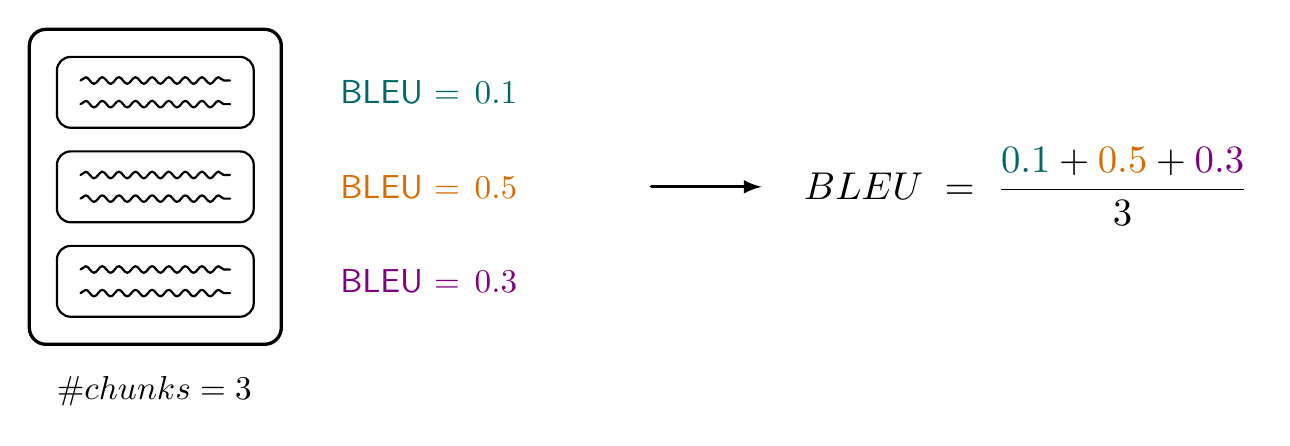
\begin{tikzpicture}[line join=round,line cap=round, >=latex, font=\sffamily]

% --- Left black container with three chunks ---
\draw[black, very thick, rounded corners=6pt]
  (-0.2,3.6) rectangle (3.0,-0.4);

% three inner rounded rectangles
\foreach \y in {2.8,1.6,0.4}{
  \draw[black, thick, rounded corners=5pt] (0.15,\y+0.45) rectangle (2.65,\y-0.45);
  % squiggle inside
  \draw[black, thick, decorate, decoration={snake,amplitude=1.2pt,segment length=6pt}]
    (0.45,\y-0.15) -- (2.35,\y-0.15);
  \draw[black, thick, decorate, decoration={snake,amplitude=1.2pt,segment length=6pt}]
  (0.45,\y+0.15) -- (2.35,\y+0.15);
}

% --- Colored BLEU labels next to each chunk ---
\node[anchor=west, text=teal!80!black, scale=1.2]  at (3.6,2.8) {BLEU $=\,0.1$};
\node[anchor=west, text=orange!85!black, scale=1.2] at (3.6,1.6) {BLEU $=\,0.5$};
\node[anchor=west, text=violet, scale=1.2]         at (3.6,0.4) {BLEU $=\,0.3$};

% --- n_chunks = 3 (black) ---
\node[anchor=west, text=black, scale=1.2] at (0.0,-1.0) {$\#\text{ chunks}=3$};

% --- Arrow to the right and mean BLEU expression ---
\draw[black, very thick, ->, >=latex] (7.7,1.6) -- (9.1,1.6);

\node[anchor=west, text=black, scale=1.4] at (9.3,1.6)
  {$\varnothing\ \text{BLEU} \;=\; \displaystyle
   \frac{\textcolor{teal!80!black}{0.1}+\textcolor{orange!85!black}{0.5}+\textcolor{violet}{0.3}}{3}$};

\end{tikzpicture}
}
  \caption[Computation of the mean \ac{bleu} score over chunks]{Computation of the mean \ac{bleu} score over three text chunks of a text.}
  \label{fig:mean-bleu}
\end{figure}
